\documentclass{article}
\usepackage[spanish]{babel}
	\deactivatetilden
\spanishdecimal{.}
\addto\captionsspanish{\def\tablename{Tabla}}
\addto\captionsspanish{\def\listtablename{\'Indice de tablas}}
\usepackage[numbers,sort&compress]{natbib}
\usepackage[T1]{fontenc}
\usepackage[utf8]{inputenc}
\usepackage{graphicx}
\usepackage{url}
\usepackage{graphicx}
\graphicspath{{Figuras/}}
\usepackage[numbers,sort&compress]{natbib}
\usepackage[clearempty,pagestyles]{titlesec}
\usepackage{anysize}
\usepackage{xcolor, colortbl}
\usepackage{array, multirow, multicol}
\usepackage{enumerate} 

\def\baselinestretch{1.5}
\papersize{27.9cm}{21.5cm} 
\marginsize{2cm}{2cm}{1cm}{1cm}

\title {Búsqueda Local}
\author{Julio Garc\'ia}
\pagestyle{empty}

\pagestyle{empty}
\begin{document}
	\renewcommand{\listtablename}{Índice de tablas}
	\renewcommand{\tablename}{Cuadro}
	\maketitle
	
	\section{Introducción}
	En el presente trabajo se busca como objetivo principal la implementación de una búsqueda local en un espacio de tres dimensiones. En este caso se persigue el objetivo de encontrar el máximo valor que una función de dos variables $g(x,y)$ alcance en una cuadrícula con las condiciones $-3 \leq x$, $y \leq 3$. 

	\section{Desarrollo}
	En este trabajo se realiza la implementación de una búsqueda local en un espacio de tres dimensiones, evaluando una función de dos variables. El fin principal de esta búsqueda local es encontrar el máximo valor que la función de dos variables g(x,y) alcanza en una cuadrícula con las condiciones  $-3 \leq x$, $y \leq 3$.\\
	Dentro de los supuestos tomados en cuenta se encuentran:
	\begin{enumerate}
		\item La evaluación no se puede salir de la región  $-3 \leq x$, $y \leq 3$, se restringen los movimientos que exceden esa cuadricula a que se mantengan en el borde de la misma.
		\item En cada iteración se va guardando la solución obtenida, y también la mejor solución encontrada, en algunos pasos ambas soluciones pueden coincidir lo cual indicaría que en esta iteración se alcanzó un mejor valor de la función y por eso se actualizó la mejor solución encontrada.
	\end{enumerate}
	La función $g(x,y)$ utilizada fue: \\
	
	$g(x,y)= sin(1000*xy)*((x + 0.5)^4 - 30 * x^2 - 20 * x + (y + 0.5)^4 - 30 * y^2 - 20 * y )/100$  \\

	
	El cambio que se tiene con respecto a la función propuesta por la Dra. Elisa Schaeffer es que se multiplica la función por el término $sin(1000*xy)$ con el fin de agregar ondas en la gráfica. Cabe mencionar que el mil surgió porque si solo pone $sin(xy)$ la búsqueda local no tiene muchos movimientos (se estanca en uno de los picos de la gráfica). A continuación se presentan las gráficas correspondientes elaboradas Python 3:\\

	\begin{figure}[h!]
		\centering
		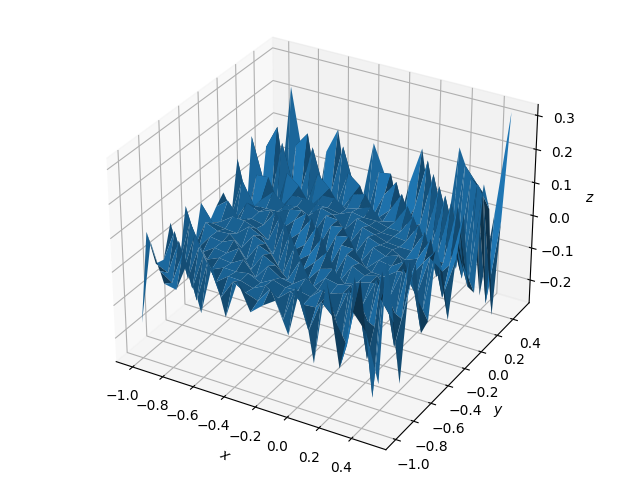
\includegraphics[width=0.7\linewidth]{Figure_1.png}
		\caption{$z=sin(1000*xy)*((x + 0.5)^4 - 30 * x^2 - 20 * x + (y + 0.5)^4 - 30 * y^2 - 20 * y )/100$}
		\label{fig:imagen1}
		
		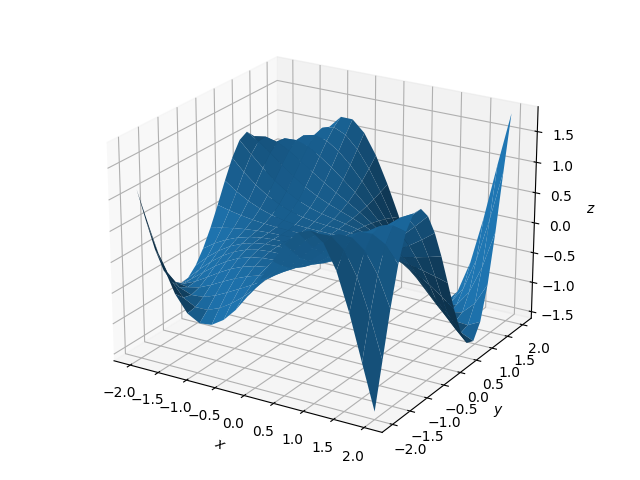
\includegraphics[width=0.7\linewidth]{Figure_2.png}
		\caption{$z=sin(xy)*((x + 0.5)^4 - 30 * x^2 - 20 * x + (y + 0.5)^4 - 30 * y^2 - 20 * y )/100$}
		\label{fig:imagen2}
	\end{figure}
\newpage
\section{Experimentación y resultados}
En esta sección se describe el ambiente computacional y los resultados obtenidos con la simulación. El código de dicha simulación fue realizado en el lenguaje computacional Python en una computadora personal con procesador 1 Intel Core i7, con memoria RAM de $16$ GB y hasta $8$ núcleos de procesamiento. Dicho código fue incorporado en el repositorio \cite{p_7}.  Se tomó como base el código de la Dra. Elisa Schaeffer \cite{p7} realizando las adecuaciones necesarias, entre las que se encuentran:

\begin{enumerate}
	\item Búsqueda ahora en función $g(x,y)$ (función de dos variables).
	\item Cuatro tipos de movimiento para la búsqueda local {IzquierdaArriba, IzquierdaAbajo, DerechaArriba, DerechaAbajo}
	\item Restringir movimientos para que no salgan de la cuadrícula $-3 \leq x$, $y \leq 3$.
	\item 	Impresión de dos marcas:
	   \begin{enumerate}	
	   	\item Estrella roja: para el punto de la mejor solución encontrada.
   		\item Diamante rosa: para el punto actual.
		\end{enumerate}

\end{enumerate}

A continuación, se presentan imágenes obtenidas, en este caso en la iteración 11 de la búsqueda local implementada la estrella coincide con el diamante. En la iteración 12 se realizó un movimiento y se muestran tanto el punto actual de la búsqueda locál así como el punto de la mejor solución obtenida a lo largo del proceso.

	\begin{figure}[h!]
	\centering
	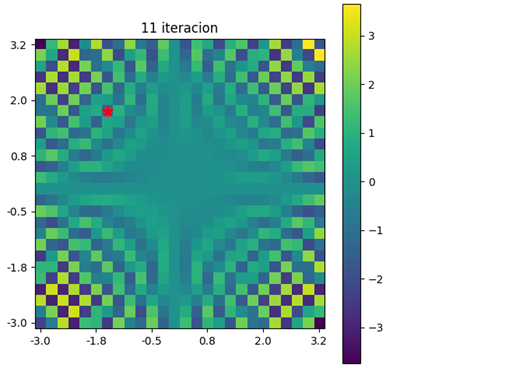
\includegraphics[width=0.7\linewidth]{Figure_3.png}
	\caption{Iteración 11}
	\label{fig:imagen3}

	\end{figure}

	\begin{figure}[h!]
	\centering
	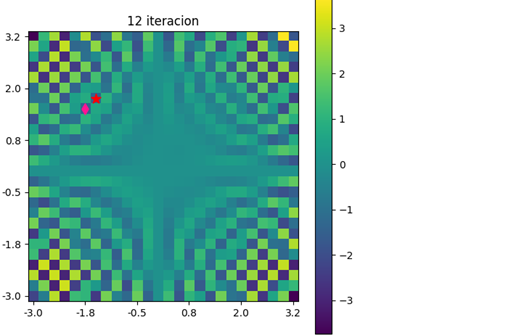
\includegraphics[width=0.7\linewidth]{Figure_4.png}
	\caption{Iteración 12}
	\label{fig:imagen4}
	\end{figure}
\newpage

\section{Conclusiones}
A continuación, se presentan las conclusiones basados en los resultado y el comportamiento de la búsqueda local implementada.
\begin{enumerate}
\item Dependiendo del tipo se función en la que se desee buscar, la búsqueda local propuesta se puede estancar (por ejemplo, cuando sólo ponemos en la función $sin(xy)$ en lugar de $sin(100xy)$.
\item La definición del paso puede también ayudar a salir de un máximo de la gráfica, un paso mas grande podría ayudar a que en algún momento de busque en una región totalmente diferente.
\item El aumentar la cantidad de iteraciones puede ayudar también a ir a buscar en otra región totalmente diferente, sin embargo con paso pequeño se puede tardar mucho en llegar a esa otra región.
\end{enumerate}

\bibliography{Biblio}
\bibliographystyle{plainnat}

\end{document}